\documentclass{standalone}
%
\usepackage{tikz,xcolor}
\usetikzlibrary{shapes.geometric,arrows,positioning,fit}
\tikzstyle{arrow} = [thick,->,>=stealth]

\begin{document}
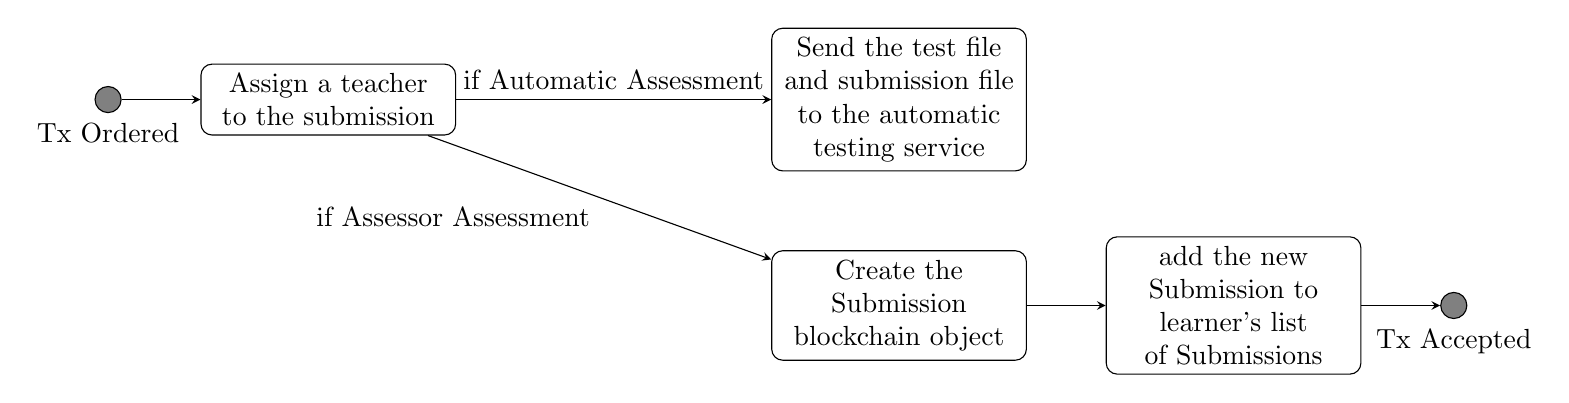
\begin{tikzpicture}[>=stealth,every node/.style={shape=rectangle,draw,rounded corners},]
    % create the nodes
    \node (start)[shape=circle, fill=gray, label=below:Tx Ordered] {};
    \node (c1) [right = and of start, text width=3cm, align=center]{Assign a teacher to the submission};
    \node (auto1) [right = and 4cm of c1, text width=3cm, align=center]{Send the test file and submission file to the automatic testing service};
    \node (ass1) [below =of auto1, text width=3cm, align=center]{Create the Submission blockchain object};
    \node (ass2) [right =of ass1, text width=3cm, align=center]{add the new Submission to learner's list of Submissions};
    \node (stop2)[right = of ass2, shape=circle, fill=gray, label=below:Tx Accepted] {};    
    % connect the nodes
    \draw[->] (start) to (c1);
    \draw[->] (c1) -- node[draw=none, anchor=south] {if Automatic Assessment} (auto1);
    \draw[->] (c1) -- node[draw=none, anchor=north east] {if Assessor Assessment} (ass1);
    \draw[->] (ass1) to (ass2);
    \draw[->] (ass2) to (stop2);    
\end{tikzpicture}
\end{document}
